% ============================================================
%  DARES Electronics - Project Structure Proposal
%  Compile with pdfLaTeX (Overleaf default). Two passes for refs.
% ============================================================
\documentclass[10pt,a4paper]{article}

% ---------- page ----------
\usepackage[margin=17mm,top=15mm,bottom=16mm]{geometry}
\usepackage[T1]{fontenc}
\usepackage[utf8]{inputenc}
\IfFileExists{sourcesanspro.sty}
  {\usepackage[default,semibold]{sourcesanspro}}
  {\IfFileExists{lmodern.sty}{\usepackage{lmodern}}{\usepackage{helvet}}%
   \renewcommand*\familydefault{\sfdefault}}
\usepackage{microtype}

% ---------- core ----------
\usepackage{xcolor,graphicx,booktabs,array,tabularx,multicol,ragged2e,enumitem,titlesec}
\usepackage[most]{tcolorbox}
\usepackage{tikz}
\usetikzlibrary{positioning,arrows.meta,fit,backgrounds,calc,shapes.misc}
\usepackage{fancyhdr,lastpage,needspace}
\usepackage[colorlinks=true,linkcolor=ink,urlcolor=blue,citecolor=ink]{hyperref}
\IfFileExists{fontawesome5.sty}{\usepackage{fontawesome5}}{\providecommand{\faIcon}[2][]{}}

% ---------- palette ----------
\definecolor{ink}{HTML}{2B2B2A}
\definecolor{muted}{HTML}{6E6E6A}
\definecolor{rule}{HTML}{D8D6D0}
\definecolor{purple}{HTML}{6B5FD1}
\definecolor{coral}{HTML}{D9582F}
\definecolor{teal}{HTML}{1E9E76}
\definecolor{blue}{HTML}{2F7FD1}
\definecolor{amber}{HTML}{B8730F}
\definecolor{slate}{HTML}{5A6B7A}
\definecolor{paper}{HTML}{FBFAF7}

% ---------- typography ----------
\color{ink}
\setlength{\parindent}{0pt}
\setlength{\parskip}{4pt}
\titleformat{\section}{\Large\bfseries\color{ink}}{}{0pt}{}[{\color{rule}\titlerule[0.8pt]}]
\titlespacing*{\section}{0pt}{10pt}{5pt}
\titleformat{\subsection}{\normalsize\bfseries\color{muted}}{}{0pt}{\MakeUppercase}
\titlespacing*{\subsection}{0pt}{7pt}{2pt}
\setlist{nosep,leftmargin=1.25em,itemsep=1pt}
\renewcommand{\arraystretch}{1.18}

% ---------- header / footer ----------
\pagestyle{fancy}\fancyhf{}
\renewcommand{\headrulewidth}{0pt}
\fancyhead[L]{\footnotesize\color{muted}DARES Electronics \textbullet{} Project structure proposal}
\fancyhead[R]{\footnotesize\color{muted}Internal \textbullet{} for officer sign-off}
\fancyfoot[C]{\footnotesize\color{muted}\thepage\ / \pageref{LastPage}}

% ---------- reusable boxes ----------
\newtcolorbox{summarybox}{enhanced,colback=paper,colframe=ink,boxrule=0.6pt,arc=2pt,
  left=8pt,right=8pt,top=6pt,bottom=6pt,fonttitle=\bfseries,title=Summary}
\newtcolorbox{decisionbox}{enhanced,colback=coral!6,colframe=coral,boxrule=0.6pt,arc=2pt,
  left=8pt,right=8pt,top=6pt,bottom=6pt,fonttitle=\bfseries\color{white},colbacktitle=coral,
  title=Decisions requested at this meeting}
\newtcolorbox{callout}[1][purple]{enhanced,colback=#1!5,colframe=#1!5,borderline west={2.5pt}{0pt}{#1},
  arc=0pt,left=8pt,right=6pt,top=4pt,bottom=4pt,boxrule=0pt}

% one project = one box, colour-coded
\newtcolorbox{project}[3]{enhanced,breakable,colback=white,colframe=#2,boxrule=0.8pt,arc=3pt,
  left=8pt,right=8pt,top=6pt,bottom=6pt,
  fonttitle=\bfseries\large\color{white},colbacktitle=#2,
  title={#1\hfill\normalsize\mdseries #3},
  before skip=8pt,after skip=8pt}

% research sub-box inside a project
\newtcolorbox{research}[1]{enhanced,colback=#1!4,colframe=#1!4,arc=2pt,boxrule=0pt,
  left=7pt,right=7pt,top=4pt,bottom=4pt,fonttitle=\bfseries\color{#1},
  title={Self-directed research},before skip=5pt,after skip=2pt}

% keyword pill
\newcommand{\pill}[2]{\tcbox[on line,colback=#1!12,colframe=#1!12,arc=6pt,boxrule=0pt,
  left=4pt,right=4pt,top=1pt,bottom=1pt,fontupper=\footnotesize]{#2}}

% inline label
\newcommand{\lbl}[1]{{\footnotesize\bfseries\color{muted}\MakeUppercase{#1}}}
% milestone item label
\newcommand{\M}[1]{{\bfseries\color{muted}M#1}}

% ============================================================
\begin{document}

% ---------- title block ----------
{\color{muted}\footnotesize Drone Aviation Racing \& Engineering Society \textbullet{} University of Melbourne}\\[2pt]
{\Huge\bfseries DARES Electronics}\\[2pt]
{\LARGE Project structure proposal}\\[6pt]
{\color{muted}Prepared by David Shmail \textbullet{} 14 September 2026 \textbullet{} v1 for internal sign-off}

\vspace{8pt}
\begin{summarybox}
Ten people answered the onboarding form. Flight control dominates their interest (6 of 9 unique respondents), three people want to lead, and three software-oriented members have no hardware home yet. Assuming half the team commits weekly hours, we can sustain \textbf{six projects of two to three people}: the three that already exist, widened where the form asks for it, plus three new ones that give the software people a product, split the flight-control overflow, and formalise the test bench. Together they own every electrical function needed to fly, and each produces numbers the FDR depends on. Members who have not submitted the form are listed but unallocated.
\end{summarybox}

% ============================================================
\section{What the form told us}

\begin{center}
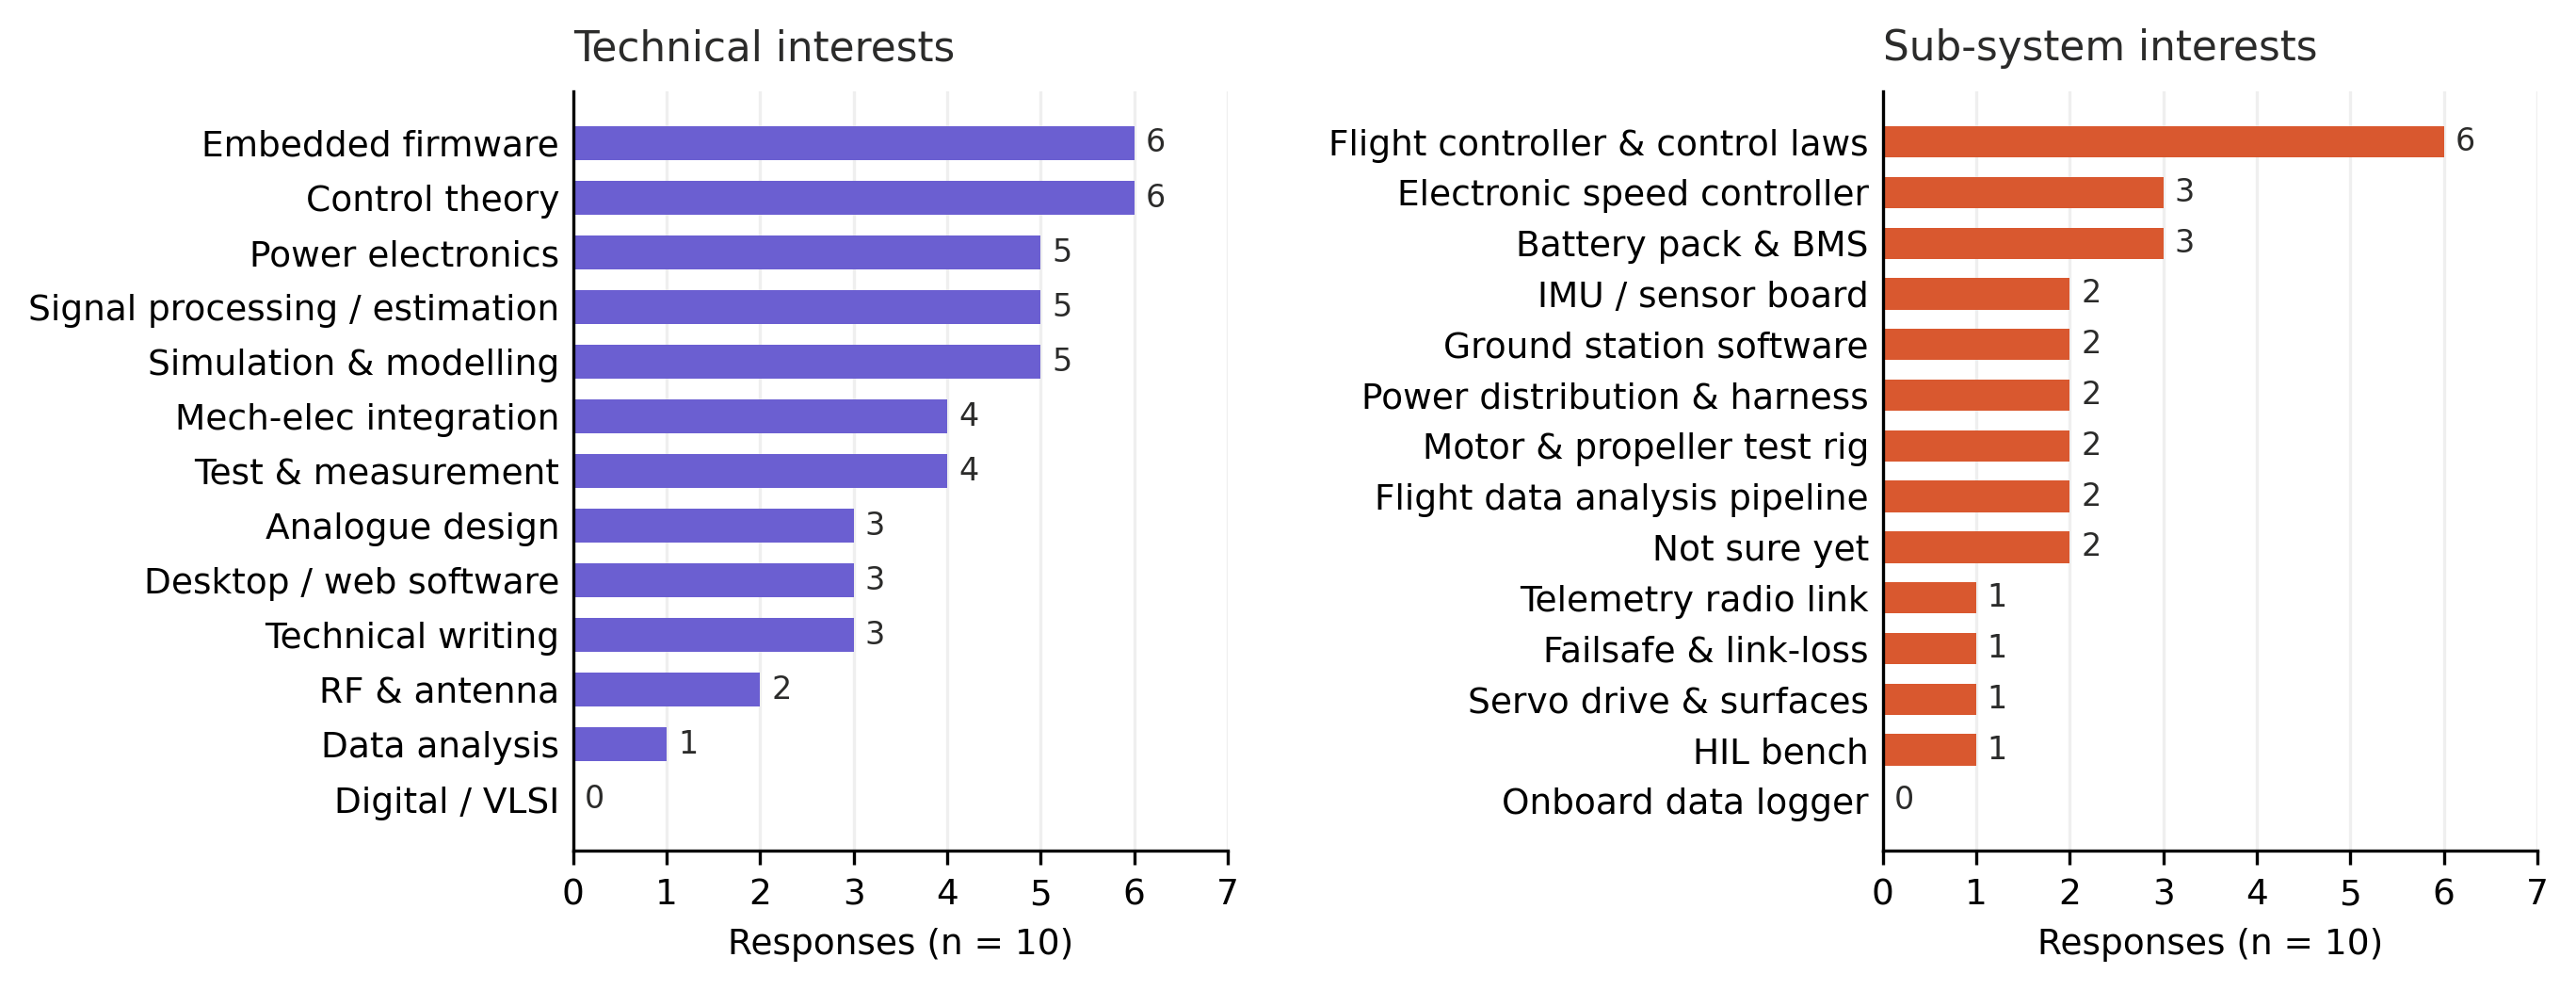
\includegraphics[width=0.98\textwidth]{figures/form_interests.png}
\end{center}
\vspace{-4pt}
\begin{multicols}{2}
\begin{itemize}[itemsep=2pt]
  \item \textbf{Flight control is the gravity well.} Six people chose it. One project cannot hold that many; it splits into control and estimation.
  \item \textbf{Three leads, three existing projects.} Rohan (flight control), Jayden (ESC), Changhan (BMS). This is the backbone.
  \item \textbf{Three software people, no home.} Wenrui, Leah and Yifei picked data pipeline, ground station and ``put me where I'm useful''.
  \item \textbf{People want the maths, not the board.} Signal processing scored 5, the IMU board 2. Estimation is a project; board design is a task inside it.
  \item \textbf{Nine of ten want the PID + IMU workshop.} That is the first workshop, not a project.
  \item \textbf{Scope reality.} Roughly 12 active members, half reliably present: six reliable engineers. Six projects of two is the ceiling.
\end{itemize}
\end{multicols}
\vspace{-6pt}
\begin{center}
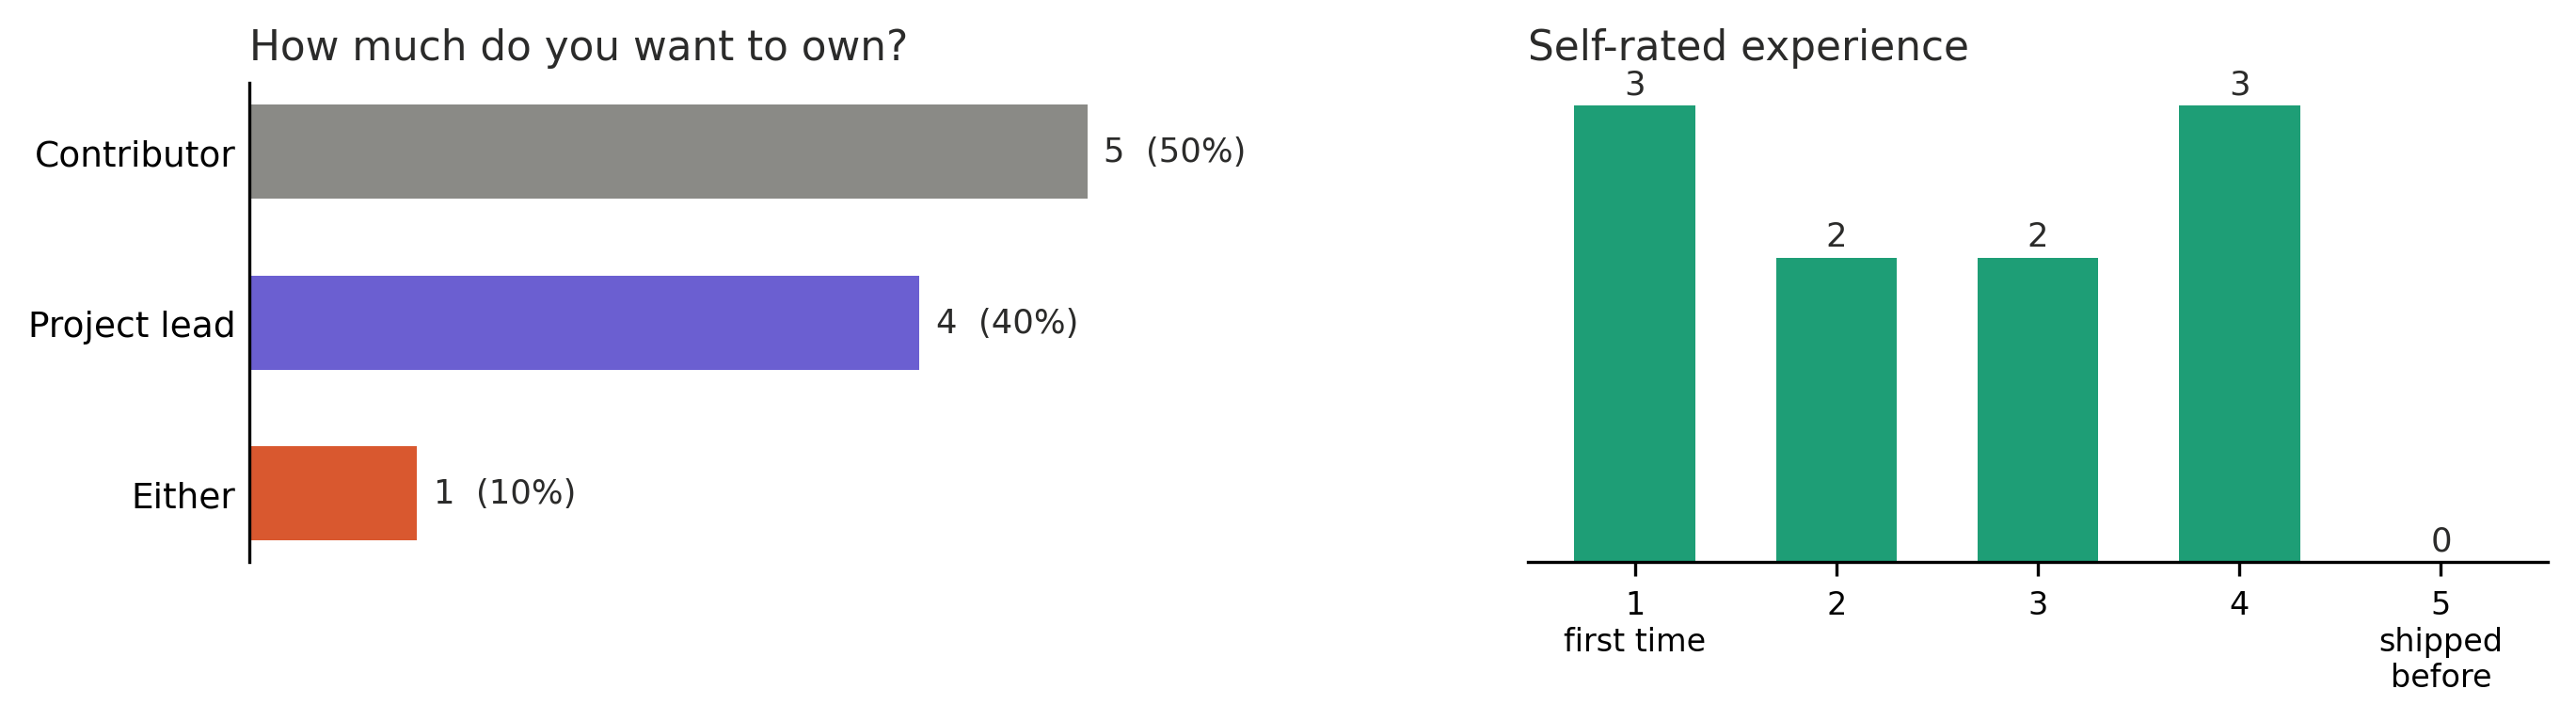
\includegraphics[width=0.82\textwidth]{figures/form_ownership_experience.png}
\end{center}

% ============================================================
\clearpage\section{Proposed structure}

\begin{center}
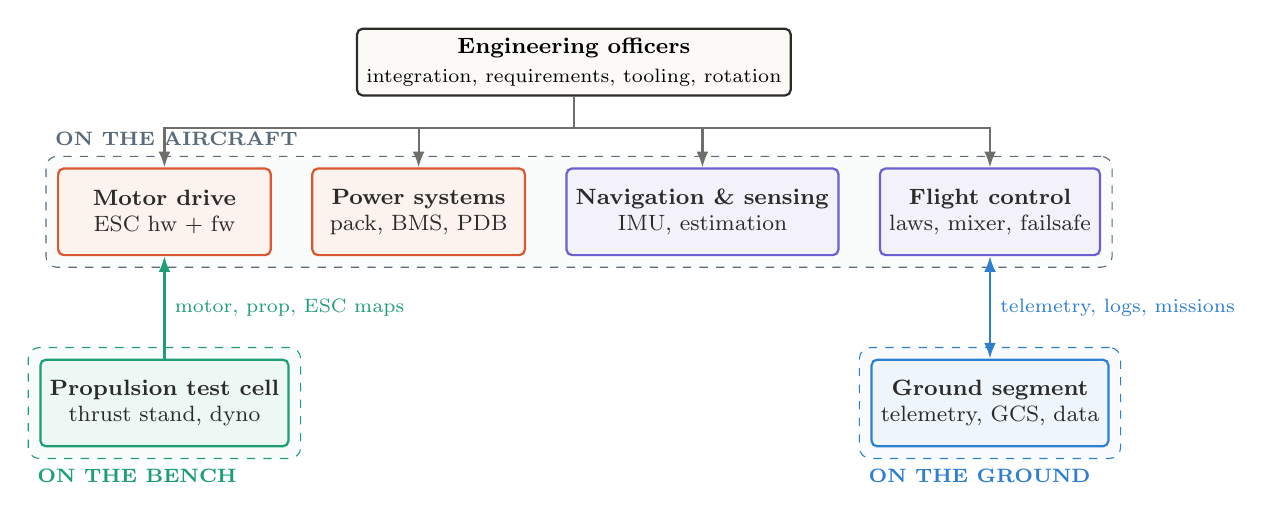
\begin{tikzpicture}[
  font=\footnotesize,
  node distance=6mm and 5mm,
  box/.style={draw=#1,fill=#1!8,rounded corners=2pt,thick,minimum height=11mm,minimum width=27mm,align=center,text=ink},
  officer/.style={draw=ink,fill=paper,rounded corners=2pt,thick,minimum height=8mm,minimum width=44mm,align=center},
  grp/.style={draw=#1,dashed,rounded corners=4pt,inner sep=4pt,fill=#1!3},
  arr/.style={-{Latex[length=2mm]},thick,color=muted},
  lblt/.style={font=\scriptsize\bfseries,text=#1}
]
\node[officer] (off) {\textbf{Engineering officers}\\[1pt]{\scriptsize integration, requirements, tooling, rotation}};

\node[box=coral, below=9mm of off, xshift=-52mm] (md) {\textbf{Motor drive}\\ESC hw + fw};
\node[box=coral, right=of md] (ps) {\textbf{Power systems}\\pack, BMS, PDB};
\node[box=purple, right=of ps] (ns) {\textbf{Navigation \& sensing}\\IMU, estimation};
\node[box=purple, right=of ns] (fc) {\textbf{Flight control}\\laws, mixer, failsafe};

\node[box=teal, below=13mm of md] (tc) {\textbf{Propulsion test cell}\\thrust stand, dyno};
\node[box=blue, below=13mm of fc] (gs) {\textbf{Ground segment}\\telemetry, GCS, data};

\begin{scope}[on background layer]
  \node[grp=slate, fit=(md)(ps)(ns)(fc), label={[lblt=slate,anchor=south west]north west:ON THE AIRCRAFT}] {};
  \node[grp=teal, fit=(tc), label={[lblt=teal,anchor=north west]south west:ON THE BENCH}] {};
  \node[grp=blue, fit=(gs), label={[lblt=blue,anchor=north west]south west:ON THE GROUND}] {};
\end{scope}

\draw[arr] (off.south) -- ++(0,-4mm) -| (md.north);
\draw[arr] (off.south) -- ++(0,-4mm) -| (ps.north);
\draw[arr] (off.south) -- ++(0,-4mm) -| (ns.north);
\draw[arr] (off.south) -- ++(0,-4mm) -| (fc.north);
\draw[arr,teal] (tc.north) -- node[right,font=\scriptsize,text=teal]{motor, prop, ESC maps} (md.south);
\draw[arr,blue,{Latex[length=2mm]}-{Latex[length=2mm]}] (gs.north) -- node[right,font=\scriptsize,text=blue]{telemetry, logs, missions} (fc.south);
\end{tikzpicture}
\end{center}

\subsection{Staffing from the form}

\begin{tabularx}{\textwidth}{@{}l>{\RaggedRight}X >{\RaggedRight}p{2.6cm} >{\RaggedRight}p{3.4cm} >{\RaggedRight}p{2.9cm}@{}}
\toprule
\textbf{\#} & \textbf{Project and scope} & \textbf{Lead} & \textbf{Members} & \textbf{Status}\\
\midrule
1 & \textbf{Flight control} -- control laws, mixer, failsafe logic, HIL & Rohan Lynch & Nicholas Tran, Alfred Wang & existing\\
2 & \textbf{Motor drive} -- ESC hardware and firmware, commutation, FOC & Jayden Filleul & \emph{needs members} & existing\\
3 & \textbf{Power systems} -- pack, BMS, power distribution, harness, safety switch & Changhan Zhang & Alfred Wang (shared) & existing, widened\\
4 & \textbf{Navigation \& sensing} -- IMU/sensor board, filtering, state estimation & \emph{TBD} & Yifei Sun, Nicholas Tran (shared) & new\\
5 & \textbf{Ground segment} -- telemetry link, ground station, logging, data pipeline & \emph{TBD} & Wenrui Chen, Leah Chen & new\\
6 & \textbf{Propulsion test cell} -- thrust stand, dyno, motor/prop/ESC characterisation & \emph{TBD} & Zhen Rong (Drew) Fong & new; absorbs the test bench repo\\
\bottomrule
\end{tabularx}

\vspace{4pt}
\begin{callout}[slate]
\textbf{Officers, floating across all projects:} Jinghan Li (engineering officer) and David Shmail (systems and software, integration, tooling). Integration and requirements traceability are officer responsibilities, not a project; rotating members through them later is how we build system-level awareness.
\end{callout}

\begin{callout}[amber]
\textbf{Not yet allocated -- form not submitted (13):} Amelia Zhu, Arshaan Khan, Ash Zhang, Dhirendra Singh, Harry Nguyen, Jiarong Chen, Joshua Pacifici, Kieren Lim, Mahin Shams, Shangrui Wu, Wen Gan, Zak Wan Ullok, Zixi Chen. They are placed the moment they submit the form; until then they attend the general meeting and workshops. Motor drive and the test cell are the first two projects newcomers should be steered toward: hands-on, least dependent on prior theory, and short of people.
\end{callout}

% ============================================================
\section{The projects}

Each project is described the same way: purpose, what it delivers as a black box, milestones in order (not on a timeline), a broad and adoptable tool stack, what we can hand the team next week, and a self-directed research brief that names the early architectural decisions the team is expected to make for itself.

% ---------------------------------------------------------------------------
\Needspace{9\baselineskip}\begin{project}{1 \, Flight control}{purple}{Rohan Lynch \textbullet{} Nicholas Tran \textbullet{} Alfred Wang}
\lbl{Purpose} \; Keep the aircraft where it is told to be, recover it when things go wrong, and produce the flight behaviour the FDR predicted.

\lbl{Black box} \; \textit{In:} state estimate, pilot or mission setpoints, link status. \; \textit{Out:} motor and servo commands, flight mode, failsafe actions, logged controller states.

\lbl{Milestones} \;
\M{0} baseline platform chosen, simulator running \;$\rightarrow$\;
\M{1} rate loop stable on the bench (HIL) \;$\rightarrow$\;
\M{2} attitude loop and mixer, first flight on a COTS flight controller \;$\rightarrow$\;
\M{3} failsafe and mission modes \;$\rightarrow$\;
\M{4} predicted-vs-measured flight characterisation for the FDR.

\lbl{Stack} \; PX4 or ArduPilot as reference implementation; C/C++ on an STM32-class autopilot; MATLAB/Simulink or Python for the plant model; SITL/HIL (jMAVSim, Gazebo, Simulink) before any flight.

\lbl{Next week} \; Pick the baseline (COTS autopilot to fly on vs. what we write ourselves); get a fixed-wing SITL running end to end; list every rule in the competition document that touches control or emergency procedures.

\begin{research}{purple}
\pill{purple}{cascaded PID} \pill{purple}{rate loop} \pill{purple}{TECS} \pill{purple}{L1 / NPFG guidance} \pill{purple}{control allocation} \pill{purple}{LQR} \pill{purple}{MPC} \pill{purple}{gain scheduling} \pill{purple}{HIL / SITL} \pill{purple}{airworthiness}

\smallskip
\begin{multicols}{2}\RaggedRight
\textbf{Start here.}
\begin{itemize}
  \item PX4 developer docs, control architecture: \href{https://docs.px4.io/main/en/flight_stack/controller_diagrams.html}{docs.px4.io}
  \item ArduPilot developer wiki: \href{https://ardupilot.org/dev/}{ardupilot.org/dev}
  \item Beard \& McLain, \emph{Small Unmanned Aircraft}: \href{https://github.com/byu-magicc/mavsim_public}{mavsim companion code}
  \item Brian Douglas, control system lectures (YouTube) for intuition on every loop we will tune
  \item acados, real-time MPC toolkit: \href{https://github.com/acados/acados}{acados on GitHub}
\end{itemize}
\columnbreak
\textbf{Decide early.}
\begin{itemize}
  \item Fly on PX4/ArduPilot and study it, or write our own stack? (Suggest: fly on COTS, replace pieces as we prove ours.)
  \item Fixed-wing control structure: classical cascaded loops first; MPC/LQR as R\&D once a validated model exists.
  \item How the plant model is obtained: from the test cell and nav team, or identified in flight?
  \item What ``failsafe'' means for the aid mission: return, loiter, or land in place?
\end{itemize}
\end{multicols}
\end{research}
\end{project}

% ---------------------------------------------------------------------------
\Needspace{9\baselineskip}\begin{project}{2 \, Motor drive}{coral}{Jayden Filleul \textbullet{} \emph{needs members}}
\lbl{Purpose} \; Turn DC from the pack into precisely timed three-phase power, efficiently, without letting the magic smoke out.

\lbl{Black box} \; \textit{In:} bus voltage, throttle command, motor feedback. \; \textit{Out:} three-phase drive, telemetry (current, RPM, temperature), faults.

\lbl{Milestones} \;
\M{0} requirements set; a COTS ESC characterised on the test cell as the baseline \;$\rightarrow$\;
\M{1} six-step commutation spinning a motor on an evaluation board \;$\rightarrow$\;
\M{2} own PCB, revision A \;$\rightarrow$\;
\M{3} current control, protection, thermal validation \;$\rightarrow$\;
\M{4} field-oriented control as R\&D.

\lbl{Stack} \; KiCad or OrCAD; LTspice/PLECS for the power stage; STM32G4 or TI C2000 class MCU in C; SimpleFOC and VESC as open reference designs; oscilloscope with a current probe.

\lbl{Next week} \; Write the one-page requirements sheet (voltage class, current, motor Kv range, protection); buy or borrow a motor-control evaluation kit; have the test cell measure a COTS ESC so there is a number to beat.

\begin{research}{coral}
\pill{coral}{six-step} \pill{coral}{sensorless back-EMF} \pill{coral}{FOC / SVPWM} \pill{coral}{dead-time} \pill{coral}{gate driver} \pill{coral}{shunt vs inline sensing} \pill{coral}{DShot} \pill{coral}{regenerative braking} \pill{coral}{thermal derating}

\smallskip
\begin{multicols}{2}\RaggedRight
\textbf{Start here.}
\begin{itemize}
  \item VESC project, open hardware and firmware: \href{https://vesc-project.com}{vesc-project.com}
  \item SimpleFOC, the gentlest FOC introduction: \href{https://simplefoc.com}{simplefoc.com}
  \item AM32, open-source drone ESC firmware: \href{https://github.com/am32-firmware/AM32}{github.com/am32-firmware/AM32}
  \item ODrive documentation for current loop and calibration practice: \href{https://docs.odriverobotics.com}{docs.odriverobotics.com}
  \item Vendor application notes: TI \emph{sensorless FOC} and ST \emph{Motor Control SDK} user manuals
\end{itemize}
\columnbreak
\textbf{Decide early.}
\begin{itemize}
  \item Build our own ESC or fly COTS and build ours as R\&D? (Suggest: fly COTS for NFC, ship ours when the test cell says it is better.)
  \item Voltage class and current rating, driven by the pack decision from power systems.
  \item Sensorless six-step first, or straight to FOC with a position estimate?
  \item MCU family, which fixes the toolchain for the whole team.
\end{itemize}
\end{multicols}
\end{research}
\end{project}

% ---------------------------------------------------------------------------
\Needspace{9\baselineskip}\begin{project}{3 \, Power systems}{coral}{Changhan Zhang \textbullet{} Alfred Wang}
\lbl{Purpose} \; Store the energy, deliver it safely on two independent buses, and always know how much is left.

\lbl{Black box} \; \textit{In:} charged cells, load demand. \; \textit{Out:} propulsion bus through the safety switch, regulated avionics rails, state of charge and pack health to the flight controller, protection trips.

\lbl{Milestones} \;
\M{0} cell chemistry and configuration chosen inside the rules; safety-switch design \;$\rightarrow$\;
\M{1} pack built, charge and discharge characterised \;$\rightarrow$\;
\M{2} BMS board: monitoring, balancing, protection \;$\rightarrow$\;
\M{3} power distribution board and harness, dual-bus integration \;$\rightarrow$\;
\M{4} state-of-charge estimation and telemetry to the flight controller.

\lbl{Stack} \; KiCad or OrCAD; LTspice; a BMS front-end evaluation board (TI BQ769x2 or ADI LTC68xx class); a logging charger; Python for cell data.

\lbl{Next week} \; Extract every battery, switch and chemistry rule from the competition document into requirement IDs; shortlist cells and series/parallel configurations; sketch the two-bus topology with the safety switch placed.

\begin{research}{coral}
\pill{coral}{passive vs active balancing} \pill{coral}{coulomb counting} \pill{coral}{OCV--SoC} \pill{coral}{equivalent-circuit model} \pill{coral}{Kalman SoC} \pill{coral}{C-rate} \pill{coral}{internal resistance} \pill{coral}{BEC / regulation} \pill{coral}{XT60 / XT90} \pill{coral}{safety switch}

\smallskip
\begin{multicols}{2}\RaggedRight
\textbf{Start here.}
\begin{itemize}
  \item Plett, \emph{Battery Management Systems} vol.\ I--II, with the free companion course: \href{https://www.coursera.org/specializations/algorithms-for-battery-management-systems}{Coursera, Algorithms for BMS}
  \item foxBMS, open-source BMS platform: \href{https://foxbms.org}{foxbms.org}
  \item TI BQ76952 datasheet and evaluation module as a worked example of a monitor IC
  \item Competition rules, Appendix I battery voltage limits and requirements S002--S004
\end{itemize}
\columnbreak
\textbf{Decide early.}
\begin{itemize}
  \item Monitor IC plus microcontroller, or fully discrete? (Suggest: monitor IC.)
  \item Passive balancing is almost certainly enough; decide and move on.
  \item Is the power distribution board part of the BMS board or separate? Separate keeps the high-current path away from the sensing.
  \item Which state-of-charge method the flight controller will trust, and what it does when the pack says ``low''.
\end{itemize}
\end{multicols}
\end{research}
\end{project}

% ---------------------------------------------------------------------------
\Needspace{9\baselineskip}\begin{project}{4 \, Navigation \& sensing}{purple}{Lead TBD \textbullet{} Yifei Sun \textbullet{} Nicholas Tran}
\lbl{Purpose} \; Turn noisy, biased sensors into a state estimate the controller can trust, and measure the airspeed and attitude the FDR must predict.

\lbl{Black box} \; \textit{In:} IMU, barometer, GPS, magnetometer, airspeed. \; \textit{Out:} attitude, angular rates, velocity, position, airspeed, wind estimate, health flags.

\lbl{Milestones} \;
\M{0} sensor selection and a test board or breakout \;$\rightarrow$\;
\M{1} raw data logged; noise and Allan-variance characterisation \;$\rightarrow$\;
\M{2} attitude filter (complementary or Mahony) validated on a bench rig \;$\rightarrow$\;
\M{3} EKF fusing GPS, baro and mag \;$\rightarrow$\;
\M{4} airspeed and wind estimation for the performance flights.

\lbl{Stack} \; Python (NumPy/SciPy) and MATLAB for design; C on the MCU; IMU evaluation boards (ICM-42688, BMI088 class); a rate table or a phone on a turntable for ground truth.

\lbl{Next week} \; Shortlist three IMUs and one GPS; write the logging plan; implement a complementary filter on any IMU we already own and plot it against integrated gyro.

\begin{research}{purple}
\pill{purple}{Allan variance} \pill{purple}{complementary / Mahony / Madgwick} \pill{purple}{error-state EKF} \pill{purple}{quaternions} \pill{purple}{gyro bias} \pill{purple}{notch filtering} \pill{purple}{vibration isolation} \pill{purple}{GNSS} \pill{purple}{pitot / airspeed}

\smallskip
\begin{multicols}{2}\RaggedRight
\textbf{Start here.}
\begin{itemize}
  \item Labbe, \emph{Kalman and Bayesian Filters in Python}: \href{https://github.com/rlabbe/Kalman-and-Bayesian-Filters-in-Python}{github.com/rlabbe}
  \item Sol\`a, \emph{Quaternion kinematics for the error-state Kalman filter}: \href{https://arxiv.org/abs/1711.02508}{arXiv:1711.02508}
  \item PX4 EKF2 tuning guide, a production estimator explained: \href{https://docs.px4.io/main/en/advanced_config/tuning_the_ecl_ekf.html}{docs.px4.io}
  \item Madgwick's original report and the Mahony filter paper; both are short
\end{itemize}
\columnbreak
\textbf{Decide early.}
\begin{itemize}
  \item Own sensor board, or use the sensors on the COTS autopilot and focus on the algorithms? (Suggest: algorithms first, board second.)
  \item Complementary filter for the first flights; EKF once there is ground truth to validate against.
  \item Where the estimator runs: on the autopilot, or on a separate processor talking over a bus?
  \item Ground-truth strategy: without one, no filter can be called validated.
\end{itemize}
\end{multicols}
\end{research}
\end{project}

% ---------------------------------------------------------------------------
\Needspace{9\baselineskip}\begin{project}{5 \, Ground segment}{blue}{Lead TBD \textbullet{} Wenrui Chen \textbullet{} Leah Chen}
\lbl{Purpose} \; Everything that talks to the aircraft or learns from it after landing: the radio links, the ground station, logging, and the data pipeline that turns flights into FDR evidence.

\lbl{Black box} \; \textit{In:} telemetry stream, onboard logs, mission plans. \; \textit{Out:} live dashboard and alerts, mission upload, archived flight datasets, predicted-vs-measured plots.

\lbl{Milestones} \;
\M{0} radio link and MAVLink end to end on the bench \;$\rightarrow$\;
\M{1} live telemetry dashboard \;$\rightarrow$\;
\M{2} log pipeline: raw log in, standard plots out \;$\rightarrow$\;
\M{3} mission upload and failsafe monitoring \;$\rightarrow$\;
\M{4} FDR-ready analysis of every flight.

\lbl{Stack} \; Python (pymavlink, MAVSDK, pandas); QGroundControl or Mission Planner as the baseline GCS; PlotJuggler or Foxglove for live and replayed data; SiK/RFD900 or ExpressLRS radios; Git LFS for logs.

\lbl{Next week} \; Get two telemetry radios talking with MAVLink heartbeats; define the flight log schema (what every flight must record); build a one-command script that turns a log into a first plot.

\begin{research}{blue}
\pill{blue}{MAVLink} \pill{blue}{ULog} \pill{blue}{915 MHz ISM (AU)} \pill{blue}{link budget} \pill{blue}{ExpressLRS} \pill{blue}{GCS / C2} \pill{blue}{time sync} \pill{blue}{pandas} \pill{blue}{Grafana / Influx} \pill{blue}{data provenance}

\smallskip
\begin{multicols}{2}\RaggedRight
\textbf{Start here.}
\begin{itemize}
  \item MAVLink protocol and tooling: \href{https://mavlink.io}{mavlink.io}
  \item PX4 Flight Review, the reference for what a flight report looks like: \href{https://review.px4.io}{review.px4.io}
  \item PlotJuggler: \href{https://plotjuggler.io}{plotjuggler.io} \textbullet{} Foxglove: \href{https://foxglove.dev}{foxglove.dev}
  \item ExpressLRS docs for the control link: \href{https://www.expresslrs.org}{expresslrs.org}
  \item RFDesign (Australian) long-range telemetry modems: \href{https://rfdesign.com.au}{rfdesign.com.au}
\end{itemize}
\columnbreak
\textbf{Decide early.}
\begin{itemize}
  \item Separate control and telemetry links, or one bidirectional link? (Suggest: separate; reliability over elegance.)
  \item Use QGroundControl and extend it, or write our own GCS in Python? (Suggest: QGC for flying, our own tooling for analysis.)
  \item Log format and the single schema every project must write to; this is the interface with everyone.
  \item Where the data lives: repository with LFS, or a shared drive with a manifest.
\end{itemize}
\end{multicols}
\end{research}
\end{project}

% ---------------------------------------------------------------------------
\Needspace{9\baselineskip}\begin{project}{6 \, Propulsion test cell}{teal}{Lead TBD \textbullet{} Zhen Rong (Drew) Fong}
\lbl{Purpose} \; Measure, rather than guess, what every motor, propeller and ESC combination actually does. The FDR performance predictions start here.

\lbl{Black box} \; \textit{In:} a motor, a prop, an ESC, a throttle profile. \; \textit{Out:} thrust, torque, RPM, electrical power, efficiency and temperature versus throttle; a dataset in the ground segment's schema.

\lbl{Milestones} \;
\M{0} existing bench inventoried; measurands and accuracy targets defined \;$\rightarrow$\;
\M{1} thrust, torque, RPM and electrical DAQ working and calibrated \;$\rightarrow$\;
\M{2} first full motor and propeller map \;$\rightarrow$\;
\M{3} automated throttle sweeps and ESC efficiency \;$\rightarrow$\;
\M{4} dataset feeding the FDR propulsion model.

\lbl{Stack} \; Load cells with an ADC front end; RPM (optical or back-EMF); current and voltage sensing; an Arduino or STM32 DAQ; Python for acquisition and plotting; the Tyto Robotics stands as the commercial reference.

\lbl{Next week} \; Photograph and list every part of the current bench; write the measurement list with target accuracy; run one manual test on any motor to find out what breaks.

\begin{research}{teal}
\pill{teal}{static thrust} \pill{teal}{Kv / Kt} \pill{teal}{propeller coefficients $C_T$, $C_P$} \pill{teal}{advance ratio} \pill{teal}{load-cell calibration} \pill{teal}{DAQ sampling} \pill{teal}{uncertainty budget} \pill{teal}{test procedure} \pill{teal}{safety cage}

\smallskip
\begin{multicols}{2}\RaggedRight
\textbf{Start here.}
\begin{itemize}
  \item UIUC propeller database, the standard for measured prop data: \href{https://m-selig.ae.illinois.edu/props/propDB.html}{m-selig.ae.illinois.edu}
  \item APC propeller performance data: \href{https://www.apcprop.com/technical-information/performance-data/}{apcprop.com}
  \item Tyto Robotics thrust-stand documentation as a design reference: \href{https://www.tytorobotics.com}{tytorobotics.com}
  \item eCalc for quick sanity checks on motor and prop pairings: \href{https://www.ecalc.ch}{ecalc.ch}
\end{itemize}
\columnbreak
\textbf{Decide early.}
\begin{itemize}
  \item Fix the existing bench or rebuild it around a proper load-cell arrangement?
  \item Static thrust only, or plan for a wind-tunnel or car-mounted dynamic test later?
  \item What the test procedure is, written down, before the first ``real'' data is taken.
  \item The data schema, agreed with the ground segment, so every dataset is comparable.
\end{itemize}
\end{multicols}
\end{research}
\end{project}




% ---------------------------------------------------------------------------
\Needspace{9\baselineskip}\begin{project}{7 \, Autonomy \& Reinforcement Learning}{amber}{Shangrui Wu \textbullet{} \emph{needs members}}

\lbl{Purpose} \;
Develop and evaluate learning-based autonomy for the fixed-wing UAV.

\lbl{Black box} \;
\textit{In:} aircraft state estimate, mission objectives, runway information,
environment observations.
\;
\textit{Out:} high-level flight commands, trajectory or guidance targets,
autonomous flight decisions, and logged training and evaluation data.

\lbl{Milestones} \;
\M{0} Gymnasium reinforcement-learning baseline completed \;$\rightarrow$\;
\M{1} custom simplified fixed-wing environment \;$\rightarrow$\;
\M{2} reinforcement learning operating in a 3D fixed-wing simulator \;$\rightarrow$\;
\M{3} custom DARES aircraft model integrated into simulation \;$\rightarrow$\;
\M{4} autonomous take-off and landing demonstrated in simulation \;$\rightarrow$\;
\M{5} robustness testing and simulation-to-real investigation.

\lbl{Stack} \;
Python; PyTorch; Gymnasium; a 3D physics-based UAV simulator; Isaac Lab or MuJoCo for 3D reinforcement-learning experiments; PX4 or ArduPilot
SITL as the conventional flight-control baseline; NumPy and Matplotlib for
training analysis; PettingZoo as an optional multi-agent extension.

\lbl{Next week} \;
Consolidate the existing Gymnasium reinforcement-learning examples; define the
observation space, action space, reward function and termination conditions for
a simplified fixed-wing environment; identify suitable 3D simulation platforms
and decide how the reinforcement-learning layer will interface with the
conventional flight controller.

\begin{research}{amber}

\pill{amber}{reinforcement learning}
\pill{amber}{Gymnasium}
\pill{amber}{PPO}
\pill{amber}{SAC}
\pill{amber}{TD3}
\pill{amber}{fixed-wing autonomy}
\pill{amber}{custom environments}
\pill{amber}{domain randomisation}
\pill{amber}{sim-to-real}
\pill{amber}{PettingZoo / MARL (optional)}

\smallskip

\begin{multicols}{2}\RaggedRight

\textbf{Start here.}

\begin{itemize}
  \item PyTorch documentation for implementing policy and value networks:
  \href{https://pytorch.org/docs/stable/index.html}{pytorch.org}

  \item Gymnasium documentation and custom-environment tutorials:
  \href{https://gymnasium.farama.org}{gymnasium.farama.org}

  
  \item PettingZoo documentation for optional future multi-agent reinforcement
  learning:
  \href{https://pettingzoo.farama.org}{pettingzoo.farama.org}
  
  \item Isaac Lab documentation for 3D reinforcement learning, physics-based
  simulation, custom environments, and simulation-to-real development:
  \href{https://isaac-sim.github.io/IsaacLab/}{isaac-sim.github.io/IsaacLab}


\end{itemize}

\columnbreak

\textbf{Decide early.}

\begin{itemize}

  \item Define the role of reinforcement learning and its interface with the
  conventional flight controller.

  \item Define the first simplified fixed-wing environment, including
  observations, actions and rewards.

  \item Select a suitable 3D simulation platform for fixed-wing reinforcement
  learning development.

  \item Define success criteria and safety constraints for autonomous take-off
  and landing.

\end{itemize}

\end{multicols}
\end{research}
\end{project}






% ============================================================
% ---- optional: screenshot of the interface map rendered in chat ----
% Save it as figures/project_interface_map.png and uncomment:
% \begin{center}\includegraphics[width=0.85\textwidth]{figures/project_interface_map.png}\end{center}
\section{Cross-cutting}

\begin{multicols}{2}
\subsection{Integration and requirements}
Owned by the officers. One interface control document listing every connector, pinout, protocol and voltage; one requirements table mapping competition rules to IDs, projects and verification methods. Both live in the general \texttt{electronics} repository, and every project links to them rather than copying them.

\subsection{Workshops, in demand order}
PID tuning and IMU filtering (9 of 10) \textbullet{} Git and GitHub (6) \textbullet{} Motors, ESCs and LiPo safety (6) \textbullet{} Low-level C (6) \textbullet{} Bench instruments (5) \textbullet{} KiCad (4) \textbullet{} Soldering (4) \textbullet{} Rules to requirements (3). The first three are the ones to run this month; they also cover exactly what the two under-staffed projects need.

\columnbreak
\subsection{Repository structure}
One general \texttt{electronics} repository for shared material, one repository per project with an identical skeleton (\texttt{README, hardware, firmware, sim, test, docs}), and a template repository for anything new. Existing repositories are renamed, not recreated.

\subsection{Cadence}
One general meeting a week: progress, plan, problems, presented by the project leads. Design check-ins and boundary reviews between adjacent projects every few weeks. Rotation is expected and encouraged.
\end{multicols}

\begin{decisionbox}
\begin{enumerate}[leftmargin=1.5em,itemsep=2pt]
  \item Confirm the six projects and the scope of each as written above.
  \item Confirm the three leads (Rohan, Jayden, Changhan) and agree how the three vacant lead positions are filled: by nomination at the next general meeting once unallocated members have submitted the form.
  \item Confirm officers own integration and requirements, and that the interface control document is started this week.
  \item Approve the first three workshops and a date for the first one.
  \item Approve the repository restructure so each project has a home before its first task is handed out.
\end{enumerate}
\end{decisionbox}

\end{document}
